% !TeX root = ../../infdesc.tex
\hintsection{\Cref*{chGettingStarted}}
\solutionsection{\Cref*{chGettingStarted}}

Consider the following statements:

\begin{enumerate}[(1)]
\item \textit{This sentence is false.}
\item \textit{I have been far even as decided to use even go want to do more like.}
\end{enumerate}

Are they true or false? If you think about (1) for a minute or two, then you'll get into a bit of a pickle, since both `true' and `false' seem to have nonsensical consequences; and (2) doesn't make any sense, so asking whether it is true or false is pointless.

Clearly we'll be wasting our time trying to write proofs of statements like the two listed above---we need to narrow our scope to statements that we might actually have a chance of proving (or perhaps refuting)! This motivates the following (informal) definition.

\begin{definition}
\label{defProposition}
\index{proposition}
\index{truth value}
A \textbf{proposition} is a statement to which it makes sense to assign a \textbf{truth value} (which, for us, can be either \textbf{true} or \textbf{false}, and can't be both).
\end{definition}

Thus the statements given at the beginning of this section are not propositions because there is no possible way of assigning them a truth value. Note that, in \Cref{defProposition}, all that matters is that it \textit{makes sense} to say that it is true or false, regardless of whether it actually \textit{is} true or false---the truth value of many propositions is unknown, even very simple ones.

\begin{exercise}
\label{exExamplesOfPropositions}
Think of an example of (a) a true proposition; (b) a false proposition; and (c) a proposition whose truth value you don't know.
\solution{exExamplesOfPropositions}{%
\fixlistskip
\begin{enumerate}[(a)]
\item $2$ is an even number.
\item $2$ is an odd number.
\item Every even integer greater than two can be expressed as the sum of two positive prime numbers. [This is \textit{Goldbach's conjecture}, proposed in 1742 by Christian Goldbach. It a famous example of an extant \textit{open problem} in mathematics. Will you be the one to solve it?]
\end{enumerate}
}
\end{exercise}

While propositions can be formed about any topic, the kinds of propositions that we will focus on in this textbook concern \textit{mathematical objects}, such as numbers (representing quantities, differences, rates, and so on), shapes, sets and functions.

Crudely speaking, pure mathematics is done by defining mathematical objects and then finding the truth values of propositions about those objects. In reality there is far more to it than that---we don't just make definitions and form propositions at random! There is usually a motivation, such as a real-world application, a problem we're trying to solve, a structure we hope to understand, or for aesthetic reasons. However, the crude `define objects and find truth values of propositions' characterisation of pure mathematics is adequate as a starting point.

If we want to determine the truth value of a proposition, we had better agree upon a way of doing so. This is where \textit{proofs} come in.

\begin{definition}
\label{defProof}
\index{proof}
A \textbf{proof} of a true proposition is an argument that demonstrates its truth; the proof should start from what is already known or assumed to be true, should use logical steps that have been agreed upon as valid, and should be verifiable by a member of its intended target audience.
\end{definition}

There is a lot going on in the definition of a proof:
\begin{itemize}
\item Starting from what is already known or assumed to be true: before we can prove anything, we need to agree upon some basic assumptions, such as the assumption that every object is equal to itself, and build up a body of knowledge from there. Technically these basic assumptions are known as \textbf{axioms}\index{axiom}; we will not worry about these too much in the main body of the book, but an interested reader can find out more in \Cref{secZFC}.
\item Using logical steps that have been agreed upon as valid: in order to deduce the truth of new propositions, we must have a logical system of rules that tell us how to do so. In this chapter we will reason informally, but we will make our logical system precise in \Cref{chLogicalStructure}. Every proof we write can, in theory, be boiled down to a sequence of deductions made according to the rules outlined in that chapter.
\item Verifiability: a reader from a proof's intended target audience should be able to understand why each deduction made in the proof is correct without having to ask for more information. Who the target audience is depends on the context---for example, much more detail would need to be provided when writing a proof in an introductory textbook on pure mathematics (such as this one) than in a mathematical research journal article.
\end{itemize}

Results in mathematical papers and textbooks may be referred to as \textit{propositions}, but they may also be referred to as \textit{theorems}, \textit{lemmas} or \textit{corollaries} depending on their intended usage.
\begin{itemize} 
\item A \textbf{proposition}\index{proposition} is an umbrella term which can be used for any result.
\item A \textbf{theorem}\index{theorem} is a key result which is particularly important.
\item A \textbf{lemma}\index{lemma} is a result that will (most likley) be used as a step in the proof of a theorem appearing later, or as a tool for the reader to use in their own proofs.
\item A \textbf{corollary}\index{corollary} is a result which follows as an immediate consequence of a theorem.
\end{itemize}

These are not precise definitions, and they are not meant to be; but using these words appropriately helps readers work out how to read a paper. For example, if you just want to skim a paper and find its key results, you'd look for the theorems.

Right, then. Let's start proving some theorems!

\dots{}

Oh, wait a minute\dots{} we don't have anything to prove anything about yet.

That's what the rest of this chapter is for: we will preview some of the concepts that will be introduced more formally later in the book, and we will write a few `starter proofs' without worrying too much about the technicalities---for now. This will help prepare us for the more rigorous treatment of mathematical proof in the rest of the textbook.

\subsection*{Numbers}

Unsurprisingly, we will encounter numbers very often on our journey through pure mathematics. Different types of number are used for representing different kinds of quantity (amount, difference, rate, position, \dots{}) of different kinds of object (discrete, continuous, finite, infinite, \dots{}).

We will illustrate the different types of number of interest to us geometrically. To that end, here is an infinite line:
\begin{center}
\begin{tikzpicture}
\draw[latex-latex] (-5.5, 0) -- (5.5, 0) ;
\end{tikzpicture}
\end{center}
The arrows indicate that it is supposed to extend in both directions without end.

Now let's fix a point on this line, and label it `$0$':
\begin{center}
\begin{tikzpicture}
\draw[latex-latex] (-5.5, 0) -- (5.5, 0) ; 
\draw (0, 0) -- (0, 0.1) node[above] {$0$} ;
\end{tikzpicture}
\end{center}
This point can be thought of as representing the number zero. It is the point against which all other numbers will be measured. Numbers to the left of $0$ on the number line are said to be \textit{negative}, and those to the right are \textit{positive}; $0$ itself is neither positive nor negative.

Finally, let's fix a unit of length:
\begin{center}
\begin{tikzpicture}
\draw (0, 0) -- (1, 0) ; 
\foreach \x in {0,1} \draw (\x, -0.1) -- (\x, 0.1)  ;
\end{tikzpicture}
\end{center}
This unit of length will be used, amongst other things, to compare the extent to which the other numbers differ from zero.

\begin{definition}
\label{defNumberLine}
The above infinite line, together with its fixed zero point and fixed unit length, constitute the (\textbf{real}) \textbf{number line}.

The numbers represented by points on the number line are called \textbf{real numbers}.
\begin{center}
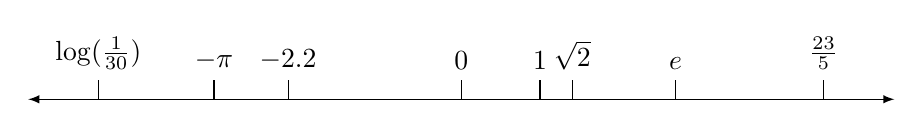
\begin{tikzpicture}
\draw[latex-latex] (-5.5, 0) -- (5.5, 0) ; 
\draw (-4.61, 0) -- (-4.61, 0.25) node[above] {$\log(\frac{1}{30})$} ;
\draw (-3.14, 0) -- (-3.14, 0.25) node[above] {$-\pi$} ;
\draw (-2.2, 0) -- (-2.2, 0.25) node[above] {$-2.2$} ;
\draw (0, 0) -- (0, 0.25) node[above] {$0$} ; 
\draw (1, 0) -- (1, 0.25) node[above] {$1$} ; 
\draw (1.41, 0) -- (1.41, 0.25) node[above] {$\sqrt{2}$} ;
\draw (2.72, 0) -- (2.72, 0.25) node[above] {$e$} ; 
\draw (4.6, 0) -- (4.6, 0.25) node[above] {$\frac{23}{5}$} ;
\end{tikzpicture}
\end{center}
~
\end{definition}

We will use the number line to provide geometric interpretations four particular types of real number: the \textit{natural numbers} (\Cref{defNaturalNumberInformal}), the \textit{integers} (\Cref{defIntegerInformal}) and the \textit{rational numbers} (\Cref{defRationalNumberInformal}).

Each of these types of number has a different character and different properties, and is used for different purposes, as we will see later in this chapter and throughout this book.

\subsubsection*{Natural numbers}

The \textit{natural numbers} are the numbers used for counting---they are the answers to questions of the form `how many'---for example, at the time of writing this paragraph, I have \textit{three} uncles, \textit{five} guinea pigs
% Shout out to Pippin, Peaches, Polly, Penelope and Plouffe
% Rest in peace, Tuft and Peeve! <3
and \textit{zero} cats.

Counting is a skill humans have had for a very long time; we know this because there is evidence of people using tally marks tens of thousands of years ago. Tally marks provide one method of counting small numbers: starting with nothing, proceed through the objects you want to count one by one, and make a mark for every object. When you are finished, there will be as many marks as there are objects. We are taught from a young age to count with our fingers; this is another instance of making tally marks, where now instead of making a mark we raise a finger.

Making a tally mark represents an \textit{increment} in quantity---that is, adding one. On our number line, we can represent an increment in quantity by moving to the right by the unit length. Then the distance from zero we have moved, which is equal to the number of times we moved right by the unit length, is therefore equal to the number of objects being counted.

\begin{definition}[Natural number]
\label{defNaturalNumberInformal}
\index{natural number}
\index{number!natural}
The \textbf{natural numbers} are the nonnegative whole numbers; they are represented by the points on the number line that can be obtained by starting at $0$ and moving right by the unit length any number of times:
\begin{center}
\begin{tikzpicture}
\draw[latex-latex] (-5.5, 0) -- (5.5, 0) ; 
\foreach \x in {0,1,2,3,4,5} \draw (\x, 0) -- (\x, 0.1) node[above] {$\x$} ;
\end{tikzpicture}
\end{center}
~
\end{definition}

The natural numbers have very important and interesting mathematical structure, and are central to the material in \Cref{chCombinatorics}. A more precise characterisation of the natural numbers will be provided in \Cref{secPeanosAxioms}, and a mathematical construction of the set of natural numbers can be found in \Cref{secZFC} (see \Cref{cnsNaturalNumbersVonNeumann}). Central to these more precise characterisations will be the notions of `zero' and of `adding one'---just like making tally marks.

\begin{aside}
Some authors define the natural numbers to be the \textit{positive} whole numbers, excluding zero. We take $0$ to be a natural number since our main use of the natural numbers will be for counting finite sets, and a set with nothing in it is certainly finite! That said, as with any mathematical definition, the choice about whether $0$ is or is not a natural number a matter of taste or convenience, and is merely a convention---it is not something that can be proved or refuted.
\end{aside}

Note that adding or multiplying two natural numbers always results in another natural number; this is to say that the natural numbers are \textit{closed} under the addition and multiplcation operations. More precisely, whenever $a$ and $b$ are natural numbers, so are $a+b$ and $ab$.

Importantly, the natural numbers are \textit{not} closed under subtraction or division: for example, $1$ and $2$ are natural numbers, but $1-2$ and $\frac{1}{2}$ are not.

\subsubsection*{Integers}

The \textit{integers} can be used for measuring the difference between two natural numbers. For example, suppose I have five apples and five bananas. Another person, also holding apples and bananas, wishes to trade. After our exchange, I have seven apples and only one banana. Thus I have \textit{two more} apples and \textit{four fewer} bananas.

Since an increment in quantity can be represented by moving to the right on the number line by the unit length, a \textit{decrement} in quantity can therefore be represented by moving to the \textit{left} by the unit length. Doing so gives rise to the integers.

\begin{definition}
\label{defIntegerInformal}
\index{integer}
\index{number!integer}
The \textbf{integers} are the whole numbers; they are represented by the points on the number line which can be obtained by starting at $0$ and moving in either direction by the unit length any number of times:
\begin{center}
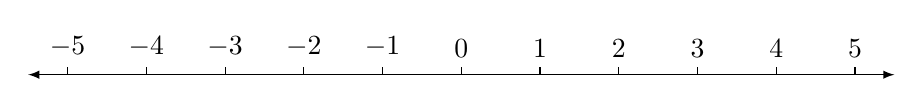
\begin{tikzpicture}
\draw[latex-latex] (-5.5, 0) -- (5.5, 0) ; 
\foreach \x in {-5,-4,-3,-2,-1,0,1,2,3,4,5} \draw (\x, 0) -- (\x, 0.1) node[above] {$\x$} ;
\end{tikzpicture}
\end{center}
~
\end{definition}

Note that just like the natural numbers, the integers are closed under addition and multiplication. They are also closed under subtraction, since whenever $a$ and $b$ are integers, so is $a-b$. However, the integers still fail to be closed under division.

The integers have such a fascinating structure that a whole chapter of this book is devoted to them---see \Cref{chNumberTheory}. This is to do with the fact that, although you can add, subtract and multiply two integers and obtain another integer, the same is not true of division. This `bad behaviour' of division is what makes the integers interesting.

One of the properties of integers that is useful in proofs is that there is always a \textit{next} one: given any integer $n$, the next integer is $n+1$, meaning that $n+1>n$ and there are no integers $k$ that satisfy the inequality $n<k<n+1$. Sometimes it is useful to be able to round a real number $x$ up or down to the next integer; this is what the \textit{floor} and \textit{ceiling} operations do.

\todo{To do: add LaTeX code for floor and ceiling}

\begin{definition}[Floor and ceiling]
\index{floor}
\index{ceiling}
Let $x$ be a real number.
\begin{itemize}
\item The \textbf{floor} of $x$ is the integer $n$ such that $n \le x < n+1$; we write $\floor{x}$ to denote the floor of $x$. Intuitively, $\floor{x}$ is the result of rounding $x$ \textit{down} to the next integer.
\item The \textbf{ceiling} of $x$ is the integer $n$ such that $n-1 < x \le n$; we write $\ceil{x}$ to denote the ceiling of $x$. Intuitively, $\ceil{x}$ is the result of rounding $x$ \textit{up} to the next integer.
\end{itemize}

The floor and ceiling operations are illustrated on the following number line diagram, with the notches representing the integers.
\begin{center}
\begin{tikzpicture}
\draw[latex-latex] (-5.5, 0) -- (5.5, 0) ; 
\foreach \x in {-5,-3,-1,1,3,5} \draw (\x, 0) -- (\x, -0.2) ;
\draw[latex-] (1.7,0) -- (1.7,0.4) node[above] {$\phantom{\lfloor}x\phantom{\rfloor}$} ;
%\draw[latex-] (1,0.2) -- (1,0.7) node[above] {$\floor{x}$} ;
%\draw[latex-] (3,0.2) -- (3,0.7) node[above] {$\ceil{x}$} ;
\draw (1,-0.1) node[below] {$\floor{x}$} ;
\draw (3,-0.1) node[below] {$\ceil{x}$} ;
\end{tikzpicture}
\end{center}
\end{definition}

\begin{example}
Some examples of floors and ceilings of real numbers include $\floor{\pi} = 3$, $\ceil{\pi} = 4$, $\floor{1.3} = 1$ and $\ceil{1.3} = 2$.
\end{example}

\begin{example}
Let $n$ be an integer. Then $n \le n < n+1$ and $n-1 < n \le n$, and so $\floor{n} = n = \ceil{n}$.
\end{example}

\begin{exercise}
\plan{week 1.1}{basis}
Suppose that $x$ is a real number that is not an integer. Prove that $\ceil{x} = \floor{x} + 1$.
\hintlabel{exFloorCeilingOfNonInteger}{%
Set $n = \floor{x}$ and verify that $n+1$ satisfies the definition of `ceiling'.
}%
\solution{exFloorCeilingOfNonInteger}{%
Set $n = \floor{x}$. Then $n \le x < n+1$ by definition of floor. Since $x$ is not an integer and $n$ is, we have $n \ne x$; but then $n<x<n+1$, and so $(n+1)-1 < x \le n+1$. This inequality demonstrates that $n+1$ is the ceiling of $x$, and so $\ceil{x} = n+1 = \floor{x} + 1$, as required.
}%
\end{exercise}

\begin{exercise}
\plan{week 1.1}{gevorderd}
Suppose that $x$ is a real number. Prove that $\floor{-x} = -\ceil{x}$ and $\ceil{-x} = -\floor{x}$.
\hintlabel{exFloorCeilingOfNegative}{%
Set $n = \floor{-x}$ and show that $-n$ satisfies the definition of being the ceiling of $x$; use a similar argument for the other part of the exercise.
}%
\solution{}{%
Set $n = \floor{-x}$. By definition of floor we have $n \le -x < n+1$. Multiplying through by $-1$ gives $-n \ge x > -(n+1)$, or equivalently $-n-1 < x \le -n$. Thus $-n$ satisfies the definition of being the ceiling of $x$, so that $\ceil{x} = -n = -\floor{-x}$. Hence $\floor{-x} = -\ceil{x}$, as required.

Now set $m = \ceil{-x}$. By definition of ceiling we have $m-1 < -x \le m$. Multiplying through by $-1$ and rearranging gives $-m \le x < -m+1$. Thus $\floor{x} = -m = -\ceil{-x}$, and so $\ceil{-x} = -\floor{x}$, as required.
}
\end{exercise}

\subsubsection*{Rational numbers}

Suppose I buy a pizza which is divided evenly into eight slices. A friend and I decide to share the pizza. I don't have much of an appetite, so I eat three slices and my friend eats five. Unfortunately, we cannot represent the proportion of the pizza each of us has eaten using natural numbers or integers: we each ate more than zero pizzas, but less than one pizza.

However, we're not far off: we can count the number of equal parts the pizza was split into, and of those parts, we can count how many we had. On the number line, this could be represented by splitting the unit line segments into eight equal segments, whose length we call an \textit{eighth} ($\frac{1}{8}$) of a unit. Counting eight segments is then equivalent to counting one unit, and each segment represents one slice of pizza.

\begin{center}
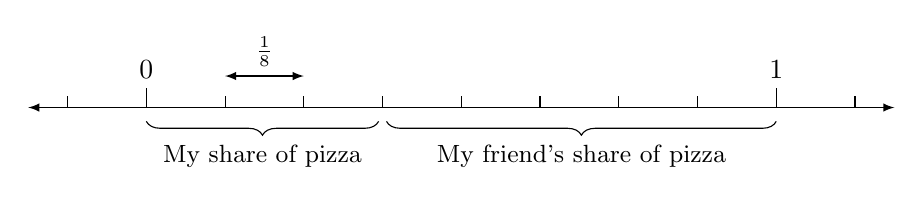
\begin{tikzpicture}
\draw[latex-latex] (-5.5, 0) -- (5.5, 0) ; 
\draw (-4, 0) -- (-4, 0.25) node[above] {$0$} ;
\draw (4, 0) -- (4, 0.25) node[above] {$1$} ;
\foreach \x in {-5,-3,-2,-1,0,1,2,3,5} {
    \draw (\x, 0) -- (\x, 0.15) ;
}
% Code for brace taken from LaTeX Stack Exchange user AboAmmar
% https://tex.stackexchange.com/a/435565
\draw[decorate, decoration={brace,mirror,amplitude=5pt,raise=5pt}] (-4,0) -- (-1.05,0) node[midway,below,yshift=-10pt] {\small My share of pizza} ;
\draw[decorate, decoration={brace,mirror,amplitude=5pt,raise=5pt}] (-0.95,0) -- (4,0) node[midway,below,yshift=-10pt] {\small My friend's share of pizza} ;
\draw[latex-latex] (-3, 0.4) -- (-2, 0.4) node[midway,above] {\small $\frac{1}{8}$} ;

\end{tikzpicture}
\end{center}

This kind of procedure gives rise to the \textit{rational numbers}.
\begin{definition}
\label{defRationalNumberInformal}
\index{rational number}
\index{number!rational}
A \textbf{rational number} is a real number that can be expressed as an integer divided by a nonzero integer; that is, $x$ is a rational number if and only if there are integers $a$ and $b$, with $b \ne 0$, such that $x = \dfrac{a}{b}$.

The representation of rational numbers on the number line is a little more involved. Given a positive integer $b$, the real number $\frac{1}{b}$ represents the length obtained by breaking up the unit length into $b$ equal parts:
\begin{center}
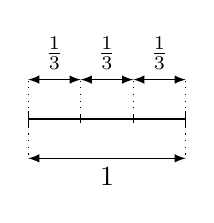
\begin{tikzpicture}
\draw (0,0) -- (2,0);
\draw[latex-latex] (0,-0.5) -- (2,-0.5) node[midway, below] {$1$} ;
\foreach \i in {0,1} \draw[dotted] (2*\i,-0.1) -- (2*\i,-0.5) ;
\draw (0,-0.1) -- (0,0.1) ;
\draw (2,-0.1) -- (2,0.1) ;
\foreach \i in {1,2} \draw (2*\i/3, -0.05) -- (2*\i/3, 0.05) ;
\foreach \i in {0,1,2,3} \draw[dotted] (2*\i/3, 0.05) -- (2*\i/3, 0.5) ;
\foreach \i in {0,1,2} \draw[latex-latex] (2*\i/3,0.5) -- (2*\i/3+2/3,0.5) node[midway,above] {$\frac{1}{3}$} ;
\end{tikzpicture}
\end{center}
The real numbers of the form $\frac{a}{b}$, where $a$ is an integer, are those obtained by starting at $0$ and moving to the left or right by $\frac{1}{b}$ units some number of times, with the direction and number of steps determined by the value of $a$:

\begin{center}
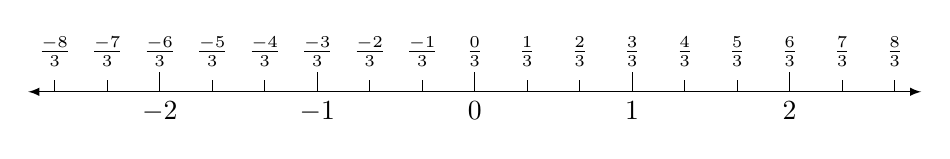
\begin{tikzpicture}
\draw[latex-latex] (-5.67, 0) -- (5.67, 0) ; 
\foreach \x in {-2,-1,0,1,2} \draw (2*\x, 0.25) -- (2*\x, 0) node[below] {$\x$} ;
\foreach \a in {-8,-7,-5,-4,-2,-1,1,2,4,5,7,8} \draw (2*\a/3, 0) -- (2*\a/3, 0.15) ;
\foreach \a in {-8,-7,-6,-5,-4,-3,-2,-1,0,1,2,3,4,5,6,7,8} {
  \draw (2*\a/3, 0.2) node[above] {\small $\frac{\a}{3}$} ;
}
\end{tikzpicture}
\end{center}

When $b<0$, we obtain the geometric interpretation of $\frac{a}{b}$ using the fact that $\frac{a}{b}=\frac{-a}{-b}$.
\end{definition}

The rational numbers are a very important example of a type of algebraic structure known as a \textit{field}, meaning that they can be added, subtracted, multiplied and divided; indeed, given integers $a,b,c,d$ with $b \ne 0$ and $d \ne 0$, we have
\[ \frac{a}{b} + \frac{c}{d} = \frac{ad+bc}{bd}, \qquad \frac{a}{b} - \frac{c}{d} = \frac{ad-bc}{bd}, \qquad \frac{a}{b} \times \frac{c}{d} = \frac{ac}{bd} \]
and when $c \ne 0$ (so that $\frac{c}{d} \ne 0$) we have
\[ \frac{a/b}{c/d} = \frac{ad}{bc} \]
The expressions on the right-hand sides of the previous four equations are fractions with integers in the numerator and denominator, and the denominators are all nonzero, so they demonstrate that the expressions on the left-hand sides of the equations are rational numbers.

Rational numbers central to several areas of mathematics, including algebraic number theory and algebraic geometry.

%\subsubsection*{Complex numbers}
%
%\todo{to students: ignore this part, we won't be covering complex numbers in 21-127 this semester}
%
%The \textbf{complex numbers} have many different characterisations, but in particular they are the solutions to polynomial equations with real coefficients. It can be proved---but doing so is outside of the scope of this textbook---that all such numbers can be expressed as the sum of a real number and a real multiple of a square root of $-1$.
%
%\todo{Complex plane}
%
%\begin{definition}
%\label{defComplexNumberInformal}
%The \textbf{complex numbers} are those that can be expressed as the sum of a real number and a real multiple of $i$, where $i$ is a fixed solution to the equation $x^2=-1$; they are represented by the points in the complex plane.
%\end{definition}
%
%\todo{Complete this subsection}

\subsection*{Sets and elements}

Fundamental to mathematics is the notion of a \textit{set}. You will find sets in every chapter of the textbook, so we will take some time to think about them now. We will not treat sets formally at this stage---for now, the following definition will suffice.

\begin{definition}[to be revised in \Cref{secSets}]
\label{defSetsPreliminary}
\lindexmmc{in}{$\in$}
A \textbf{set} is a collection of objects. The objects in the set are called \textbf{elements} of the set. When $X$ is a set and $x$ is an object, we write $x \in X$ \inlatexnb{x \textbackslash{}in X}\nindex{in}{$\in$}{element}\lindexmmc{in}{$\in$} to denote the assertion that $x$ is an element of $X$.
\end{definition}

Sets provide a convenient language for talking about objects of a certain kind without having to describe them every time, thereby making our mathematical arguments more concise and less verbose. In fact, sets are so convenient that they are the basis of the (currently) most widely used logical foundation for mathematics---we would be getting too far ahead of ourselves to delve into this now, but details can be found in \Cref{secZFC}. Sets are also interesting objects of study in their own right: we will study them in great detail in \Cref{chSets}.

Some ubiquitous examples of sets are given by sets of numbers of a given type, collectively called \textit{number sets}.

\begin{definition}[Number sets]
\label{defNumberSets}
\index{number set}
\index{set!number}
The \textbf{number sets} are defined as follows:
\begin{itemize}
\item $\Nat$\nindex{N}{$\Nat$}{set of all natural numbers} is the set of all natural numbers;
\item $\Int$\nindex{Z}{$\Int$}{set of all integers} is the set of all integers;
\item $\Rat$\nindex{Q}{$\Rat$}{set of all rational numbers} is the set of all rational numbers;
\item $\Real$\nindex{R}{$\Real$}{set of all real numbers} is the set of all real numbers.
%\item $\Cplx$\nindex{C}{$\Cplx$}{set of all complex numbers} is the set of all complex numbers
\end{itemize}
\end{definition}

\begin{aside}
Mathematics is both case-sensitive and font-sensitive, so for example it is possible to use $x$, $\mathbf{x}$, $X$, $\mathbf{X}$, $\mathbb{X}$, and $\mathcal{X}$ to refer to six different things. The font used for the number sets is called \textit{blackboard bold} \inlatex{mathbb\{...\}}\lindexmmc{mathbb}{$\mathbb{A}, \mathbb{B}, \dots$}, and is commonplace in modern mathematical texts; some texts use regular bold face (as in $\mathbf{N}, \mathbf{Z}, \mathbf{Q}, \dots$) instead.
\end{aside}

\begin{example}
By \Cref{defSetsPreliminary} and \Cref{defNumberSets}, the expression $x \in \Int$ means that $x$ is an integer, and the expression $x \not\in \Int$ means that $x$ is not an integer. Therefore, for example, the propositions $4 \in \Int$ and $\frac{5}{2} \not\in \Int$ are both true.
\end{example}

\begin{exercise}
\label{exElementsOfNumberSets}
Determine the truth values of the following propositions.
\begin{multicols}{3}
\begin{enumerate}[(a)]
\item $2 \in \Nat$
\item $-2 \in \Nat$
\item $-2 \in \Rat$
\item $\dfrac{2}{5} \in \Int$
\item $\dfrac{\sqrt{8}+\sqrt{2}}{\sqrt{8}-\sqrt{2}} \in \Rat$
\item $\pi^{\pi} \in \Rat$
\item $\sqrt{-7} \in \Real$
%\item $\sqrt{-7} \in \Cplx$
\item\label{itmNElementOfZ} $\Nat \in \Int$
\end{enumerate}
\end{multicols}
\solution{exElementsOfNumberSets}{%
\begin{enumerate}[(a)]
\item $2 \in \Nat$ is true, since it is a nonnegative whole number and can be used for counting (for example, I have $2$ eyes).
\item $-2 \in \Nat$ is false, since $-2 < 0$ but all natural numbers are nonnegative.
\item $-2 \in \Rat$ is true, since $-2 = \dfrac{-2}{1}$, which is an integer divided by a nonzero integer.
\item $\dfrac{2}{5} \in \Int$ is false, since $0<\dfrac{2}{5}<1$, meaning that $\dfrac{2}{5}$ is strictly between two consecutive integers.
\item $\dfrac{\sqrt{8}+\sqrt{2}}{\sqrt{8}-\sqrt{2}} \in \Rat$ is true: note that $\sqrt{8} = 2\sqrt{2}$, so cancelling the common factor of $\sqrt{2}$ from the numerator and denominator reveals that this number is equal to $\dfrac{2+1}{2-1} = \dfrac{3}{1}$, which is an integer divided by a nonzero integer.
\item $\pi^{\pi} \in \Rat$\dots{} OK, sorry, this is (kind of) a trick question. Whether or not $\pi^{\pi}$ is rational is an open problem.
\item $\sqrt{-7} \in \Real$ is false: the square of every real number is nonnegative, but whatever $\sqrt{-7}$ actually \textit{is},\footnote{$\sqrt{-7}$ is an example of a \textit{complex number}, which is a topic for another time.} it presumably satisfies $\sqrt{-7}^2=-7$, which is negative.
%\item $\sqrt{-7} \in \Cplx$ is true, with a caveat: $-7$ actually has two complex square roots, namely $\sqrt{7}i$ and $-\sqrt{7}i$, and it is not immediately obvious which of these the expression `$\sqrt{-7}$' refers to. But both $\sqrt{7}i$ and $-\sqrt{7}i$ are indeed complex numbers.
\item $\Nat \in \Int$ might appear true at first sight, since every natural number is indeed an integer. However, $\Nat$ is \textit{the set of all natural numbers}, which is a set, not an integer, and so the proposition $\Nat \in \Int$ is false.
\end{enumerate}
}
\vspace{-20pt}
\end{exercise}

\subsubsection*{Specifying a set}

We defined the sets in \Cref{defNumberSets} using words, which is fine if the set is easy to describe in that way, but in practice it can be very cumbersome to do so. Some other ways of specifying sets, which are usually more concise, are using \textit{lists} and \textit{set-builder notation}, described next.

\begin{itemize}
\item \textbf{Lists.}\index{list notation}
A set can be specified by simply listing its elements; the elements should be separated by commas and enclosed in $\{$curly brackets$\}$\nindex{set}{$\{ \cdots \}$}{set notation} \inlatex{\{...\textbackslash{}\}}\lindexmmc{\{\dots\textbackslash{}\}}{$\{\dots\}$}. For example, the following is a specification of a set $A$, whose elements are the natural numbers $0$, $1$, $2$, $3$, $4$ and $5$ (inclusive):
\[ A = \{ 0, 1, 2, 3, 4, 5 \} \]
Sometimes a list might be too long to write out---maybe even infinite---or the length of the list might depend on a variable. In these cases it will be convenient to use an \textbf{implied list}\index{implied list notation}, in which some elements of the list are written, and the rest are left implicit by writing an ellipsis `$\dots$' \inlatex{dots}\lindexmmc{dots}{$\dots$}. For example, the statement
\[ B = \{ 0, 1, 4, 9, 16, 25, \dots \} \]
means (most likely) that $B$ is the set whose elements are all the squares of natural numbers. Note that there is some ambiguity here, since the reader is expected to be able to figure out what pattern is suggested by the `$\dots$'.

\item \textbf{Set-builder notation.}\index{set-builder notation}
List notation is only useful when discussing small, finite sets or sets whose elements can be listed with an obvious pattern. For some sets, it is not clear what order its elements can be listed in---in fact, as we will see in \Cref{secCountableUncountableSets}, there are some sets whose elements can't be listed at all (even in an infinite list)!

To get around this, we can use \textit{set-builder notation}, which is a means of specifying a set in terms of the properties its elements satisfy. The set of all objects $x$ satisfying some property $p(x)$ is written in set-builder notation as:
\[ \setb{x}{p(x)} \quad \text{or} \quad \{ x : p(x) \} \]

An object $a$ is an element of the set $\setb{x}{p(x)}$ if and only if the property $p(x)$ is true when $a$ is substituted for $x$ in the expression $p(x)$; that is, $a \in \{ x \mid p(x) \}$ if and only if $p(a)$ is true.

For example, if $C$ is the set of all real numbers whose square is less than $9$, we could write
\[ C = \setb{x}{x \in \Real \text{ and } x^2 < 9} \]
Then $2 \in C$ since the proposition `$2 \in \Real$ and $2^2 < 9$' is true, but $4 \not\in C$ since the proposition `$4 \in \Real$ and $4^2 < 9$' is false.

A couple of variations on set-builder notation are useful:
\begin{enumerate}[(i)]
\item If $X$ is a set that has already been defined, then $\setb{x \in X}{p(x)}$ denotes the set of all elements of $X$ that satisfy the property $p(x)$. That is,
\[ \setb{x \in X}{p(x)} = \setb{x}{x \in X \text{ and } p(x)} \]

For example, the set $C$ described above could be more succinctly expressed as $\setb{x \in \Real}{x^2 < 9}$.

\item\label{itmSetBuilderNotationVariantPatternMatching} If $\text{expr}(x)$ is some expression involving the variable $x$, then $\setb{\text{expr}(x)}{p(x)}$ refers to the set of all objects that can be expressed in the form $\mathrm{expr}(x)$ for some element $x$ that satisfies the property $p(x)$. That is,
\[ \setb{\mathrm{expr}(x)}{p(x)} = \setb{y}{\text{there is an object } x \text{ such that } y=\mathrm{expr}(x) \text{ and } p(x)} \]

For example, the set $B = \{ 0, 1, 4, 9, 16, 25, \dots \}$ described above could be more succinctly expressed as $\setb{n^2}{n \in \Nat}$, since its elements are those objects of the form $n^2$ where $n$ is a natural number.
\end{enumerate}
\end{itemize}

\begin{example}
\label{exSetNotationNumberSets}
The sets $\Nat$ and $\Int$ can be described in list notation as follows:
\[ \Nat = \{ 0, 1, 2, 3, \dots \} \quad \text{and} \quad \Int = \{ \dots, {-2}, {-1}, 0, 1, 2, 3, \dots \} \]
The set $\Rat$ can be described in set-builder notation as
\[ \Rat = \dsetb{x \in \Real}{x = \dfrac{a}{b} \text{ for some } a \in \Int \text{ and } b \in \Int \text{ with } b \ne 0} \]
We could use variant \ref{itmSetBuilderNotationVariantPatternMatching} described above to express $\Rat$ more succinctly as
\[ \Rat = \dsetb{\dfrac{a}{b}}{a \in \Int \text{ and } b \in \Int \text{ with } b \ne 0} \]
\end{example}

\begin{aside}
When we want to refer to more than one object being an element of a set, we sometimes abuse notation by simply separating the variables by commas. For example, in \Cref{exSetNotationNumberSets} we could have written
\[ \Rat = \dsetb{\dfrac{a}{b}}{a,b \in \Int \text{ with } b \ne 0} \]
\end{aside}

\begin{example}
\label{exSetsSpecifyUniverses}
The set of all even integers can be written in set-builder notation as
\[ \setb{n \in \Int}{n \text{ is even}} \]
For comparison, the set of all even natural numbers can be written as
\[ \setb{n \in \Nat}{n \text{ is even}} = \{ 0, 2, 4, 6, \dots \} \]
Note that $-6$ is an element of the former set but not of the latter set, since $-6$ is an integer but is not a natural number.

Note moreover that the expression
\[ \setb{n \in \Rat}{n \text{ is even}} \]
is meaningless, since we have not defined a notion of `evenness' for rational numbers.
\end{example}


\begin{exercise}
\label{exDyadicRatioal}
\index{rational number!dyadic}
A \textbf{dyadic rational} is a rational number that can be expressed as an integer divided by a power of $2$. Express the set of all dyadic rationals using set-builder notation in at least two different ways.
\end{exercise}

Set-builder notation is useful for defining sets based on the properties they satisfy, as in \Cref{defBracketN,defIntervals} below.

\begin{restatable}{definition}{RSdefBracketN}
\label{defBracketN}
Let $n \in \Nat$. The set $[n]$ is defined by $[n] = \setb{k \in \Nat}{k < n}$.
\end{restatable}

\begin{example}
\label{exBracketN}
In list notation, we have $[1] = \{ 0 \}$, $[2] = \{ 0, 1 \}$, $[3] = \{ 0, 1, 2 \}$, $[4] = \{ 0, 1, 2, 3 \}$, and so on. Note that $[0]$ has no elements (it is \textit{empty}, a term we will define in \Cref{defInhabited}), since there are no natural numbers $k$ satisfying the inequality $k < 0$.
\end{example}

While not particularly interesting yet, sets of the form $[n]$ will be fundamental throughout \Cref{chCombinatorics}, as they are used to define the notion of a \textit{finite set}, as well as the \textit{size} of a finite set.

Intervals are particular subsets of $\Real$ that are ubiquitous in mathematics, particularly in analysis and topology.

\begin{definition}[Intervals of the real line]
\label{defIntervals}
\index{interval}
\index{open!interval}
\index{closed!interval}
\index{unbounded!interval}
\nindex{abint1}{$(a,b)$}{open interval}
\nindex{abint2}{$[a,b]$}{closed interval}
\nindex{abint3}{$(a,b]$}{half-open interval}
\nindex{abint4}{$[a,b)$}{half-open interval}
\nindex{abint5}{$(-\infty,a)$}{unbounded interval}
\nindex{abint6}{$(a,\infty)$}{unbounded interval}
Let $a,b \in \Real$. The \textbf{open interval} $(a,b)$, the \textbf{closed interval} $[a,b]$, and the \textbf{half-open intervals} $[a,b)$ and $(a,b]$ from $a$ to $b$ are defined by
\begin{align*}
\hspace{35pt} (a,b) &= \setb{x \in \Real}{a < x < b}
&
(a,b] &= \setb{x \in \Real}{a < x \le b} 
\\
\hspace{35pt} [a,b) &= \setb{x \in \Real}{a \le x < b}
&
[a,b] &= \setb{x \in \Real}{a \le x \le b}
\end{align*}
We further define the \textbf{unbounded intervals} $(-\infty, a)$, $(-\infty, a]$, $[a, \infty)$ and $(a, \infty)$ \inlatex{infty}\lindexmmc{infty}{$\infty$} by
\begin{align*}
\hspace{35pt} (-\infty,a) &= \setb{x \in \Real}{x < a}
&
(a,\infty) &= \setb{x \in \Real}{x > a}
\\
\hspace{35pt} (-\infty, a] &= \setb{x \in \Real}{x \le a} 
&
[a,\infty) &= \setb{x \in \Real}{x \ge a}
\end{align*}
\end{definition}

Note that intervals are the set of all \textit{real} numbers satisfying the defining inequality, so for example it would not be appropriate to express the set $\setb{x \in \Int}{2 \le x \le 5}$ as $[2,5]$: the former only has integers as elements, while the latter includes all real numbers from $2$ to $5$.

\begin{example}
The following illustration depicts the open interval $(-2,5)$.

\vspace{-10pt}
\begin{center}
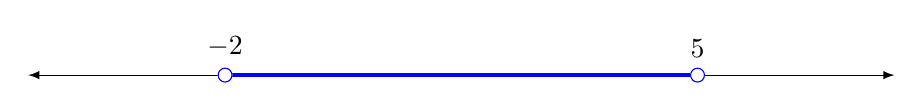
\begin{tikzpicture}
\draw[latex-latex] (-5.5,0) -- (5.5,0);
\draw[line width=1.5pt, color=blue] (-3,0) -- (3,0);
\filldraw[white](-3,0)circle[radius=2.5pt];
\draw[blue](-3,0)circle[radius=2.5pt];
\filldraw[white](3,0)circle[radius=2.5pt];
\draw[blue](3,0)circle[radius=2.5pt];
\node[at={(-3,3pt)},above]{$-2$};
\node[at={(3,3pt)},above]{$5$};
\end{tikzpicture}
\end{center}
The hollow circles $\circ$ indicate that the endpoints are not included in the interval.
\end{example}

Be warned that the use of the symbol $\infty$ is misleading, since it suggests that the symbol $\infty$ on its own has a specific meaning (or, worse, that it refers to a real number). It doesn't---it is just a symbol that suggests unboundedness of the interval in question. A less misleading way of writing $[a, \infty)$, for instance, might be $[a, {\to})$ or $\Real^{\ge a}$; however, $[a,\infty)$ is standard, so it is what we will write.

\begin{exercise}
For each of the following illustrations, find the interval that it depicts. A filled circle $\bullet$ indicates that an end-point is included in the interval, whereas a hollow circle $\circ$ indicates that an end-point is not included in the interval.

\begin{enumerate}[(a)]
\item
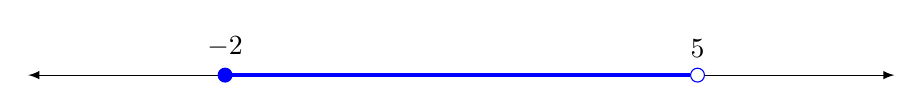
\begin{tikzpicture}
\draw[latex-latex] (-5.5,0) -- (5.5,0);
\draw[line width=1.5pt, color=blue] (-3,0) -- (3,0);
\filldraw[blue](-3,0)circle[radius=2.5pt];
\filldraw[white](3,0)circle[radius=2.5pt];
\draw[blue](3,0)circle[radius=2.5pt];
\node[at={(-3,3pt)},above]{$-2$};
\node[at={(3,3pt)},above]{$5$};
\end{tikzpicture}

\item
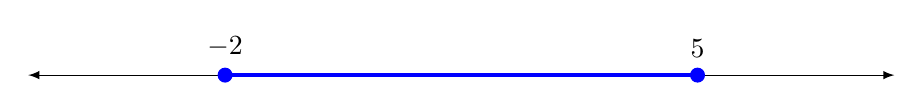
\begin{tikzpicture}
\draw[latex-latex] (-5.5,0) -- (5.5,0);
\draw[line width=1.5pt, color=blue] (-3,0) -- (3,0);
\filldraw[blue](-3,0)circle[radius=2.5pt];
\filldraw[blue](3,0)circle[radius=2.5pt];
\node[at={(-3,3pt)},above]{$-2$};
\node[at={(3,3pt)},above]{$5$};
\end{tikzpicture}


\item
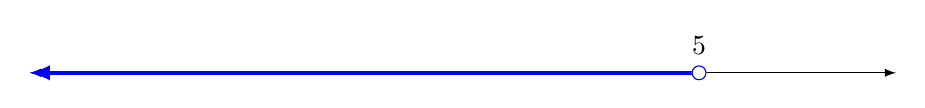
\begin{tikzpicture}
\draw[latex-latex] (-5.5,0) -- (5.5,0);
\draw[latex-, line width=1.5pt, color=blue] (-5.5,0) -- (3,0);
\filldraw[white](3,0)circle[radius=2.5pt];
\draw[blue](3,0)circle[radius=2.5pt];
\node[at={(3,3pt)},above]{$5$};
\end{tikzpicture}

\item 
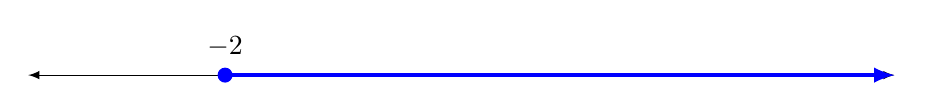
\begin{tikzpicture}
\draw[latex-latex] (-5.5,0) -- (5.5,0);
\draw[-latex, line width=1.5pt, color=blue] (-3,0) -- (5.5,0);
\filldraw[blue](-3,0)circle[radius=2.5pt];
\node[at={(-3,3pt)},above]{$-2$};
\end{tikzpicture}
\end{enumerate}
\end{exercise}

\subsection*{Getting started with proofs}

\todo{Write this}

\todo{Properties of number sets that can/can't be assumed}

\todo{Old material after this point}

\subsection*{Number bases}

Writing numbers down is something that may seem easy to you now, but it likely took you several years as a child to truly understand what was going on. Historically, there have been many different systems for representing numbers symbolically, called \textit{numeral systems}.\index{numeral system} First came the most primitive of all, tally marks, appearing in the Stone Age and still being used for some purposes today. Thousands of years and hundreds of numeral systems later, there is one dominant numeral system, understood throughout the world: the \textbf{Hindu--Arabic numeral system}.\index{numeral system!Hindu--Arabic} This numeral system consists of ten symbols, called \textit{digits}. It is a \textit{positional} numeral system, meaning that the position of a symbol in a string determines its numerical value.

In English, the \textit{Arabic numerals} are used as the ten digits:
\[ 0 \quad 1 \quad 2 \quad 3 \quad 4 \quad 5 \quad 6 \quad 7 \quad 8 \quad 9 \]
The right-most digit in a string is in the units place, and the value of each digit increases by a factor of ten moving to the left. For example, when we write `$2812$', the left-most `$2$' represents the number two thousand, whereas the last `$2$' represents the number two.

The fact that there are ten digits, and that the numeral system is based on powers of ten, is a biological accident corresponding with the fact that most humans have ten fingers. For many purposes, this is inconvenient. For example, ten does not have many positive divisors (only four: $1$, $2$, $5$ and $10$)---this has implications for the ease of performing arithmetic; a system based on the number twelve, which has six positive divisors ($1$, $2$, $3$, $4$, $6$ and $12$), might be more convenient. Another example is in computing and digital electronics, where it is more convenient to work in a \textit{binary} system, with just two digits---$0$ and $1$---which represent `off' and `on' (or `low voltage' and `high voltage'), respectively; arithmetic can then be performed directly using sequences of \textit{logic gates} in an electrical circuit.

It is therefore worthwhile to have some understanding of positional numeral systems based on numbers other than ten. The mathematical abstraction we make leads to the definition of \textit{base-$b$ expansion}.

\begin{definition}
\label{defBaseBExpansionPreliminary}
\index{base-$b$ expansion}
\index{number base}
Let $b$ be a natural number greater than $1$. The \textbf{base-$b$ expansion} of a natural number $n$ is the\footnote{The use of the word `the' is troublesome here, since it assumes that every natural number has only one base-$b$ expansion. This fact actually requires proof---see \Cref{thmBaseBExpansion}.} string $d_r d_{r-1} \dots d_0$ such that:
\begin{enumerate}[(i)]
\item $n = d_r \cdot b^r + d_{r-1} \cdot b^{r-1} + \cdots + d_0 \cdot b^0$;
\item $0 \le d_i < b$ for each $i$; and
\item If $n>0$ then $d_r \ne 0$---the base-$b$ expansion of zero is $0$ in all bases $b$.
\end{enumerate}
Certain number bases have names; for instance, the base-$2$, $3$, $8$, $10$, $12$ and $16$ expansions are respectively called \textit{binary}, \textit{ternary}, \textit{octal}, \textit{decimal}, \textit{duodecimal} (or \textit{dozenal}) and \textit{hexadecimal}.
\end{definition}

Before we look at an example of \Cref{defBaseBExpansionPreliminary} in action, let's examine the definition, which is a little terse on first sight.
\begin{itemize}
\item Condition (i) tells us that the digits in the string tell us how many of each power of $b$ are added up to obtain $n$. For example, when $b=10$, the digits from right to left tell us the units, tens, hundreds, thousands, and so on.
\item Condition (ii) tells us that the digits in a base-$b$ expansion must be less than $b$---for example, the base-$4$ digits are $0$, $1$, $2$ and $3$. If we allowed more digits then silly things would happen---for example, if `$\mathrm{X}$' were a new base-$10$ digit representing the number ten, then `$\mathrm{X}2$' and `$102$' would be different strings both representing the number one hundred and two.
\item Condition (iii) ensures that the string representing a positive number doesn't have any leading `$0$'s---otherwise, for example, `$01423$' and `$1423$' would be different strings representing the same natural number.
\end{itemize}

\begin{example}
Consider the number $1023$. Its decimal (base-$10$) expansion is $1023$, since
\[ 1023 = 1 \cdot 10^3 + 0 \cdot 10^2 + 2 \cdot 10^1 + 3 \cdot 10^0 \]
Its binary (base-$2$) expansion is $1111111111$, since
\[ 1023 = 1 \cdot 2^9 + 1 \cdot 2^8 + 1 \cdot 2^7 + 1 \cdot 2^6 + 1 \cdot 2^5 + 1 \cdot 2^4 + 1 \cdot 2^3 + 1 \cdot 2^2 + 1 \cdot 2^1 + 1 \cdot 2^0 \]
We can express numbers in base-$36$ by using the ten usual digits $0$ through $9$ and the twenty-six letters $\mathrm{A}$ through $\mathrm{Z}$; for instance, $\mathrm{A}$ represents $10$, $\mathrm{M}$ represents $22$ and $\mathrm{Z}$ represents $35$. The base-$36$ expansion of $1023$ is $\mathrm{SF}$, since
\[ 1023 = 28 \cdot 36^1 + 15 \cdot 36^0 = \mathrm{S} \cdot 36^1 + \mathrm{F} \cdot 36^0 \]
\end{example}

\begin{exercise}
Find the binary, ternary, octal, decimal, hexadecimal and base-$36$ expansions of the number $21127$, using the letters $\mathrm{A}$--$\mathrm{F}$ as additional digits for the hexadecimal expansion (representing the numbers $10$--$15$, respectively), and the letters $\mathrm{A}$--$\mathrm{Z}$ as additional digits for the base-$36$ expansion.
\end{exercise}

We sometimes wish to specify a natural number in terms of its base-$b$ expansion; we have some notation for this.

\begin{notation}
Let $b>1$. If the numbers $d_0,d_1,\dots,d_r$ are base-$b$ digits (in the sense of \Cref{defBaseBExpansionPreliminary}), then we write
\[ {d_rd_{r-1} \dots d_0}_{(b)} = d_r \cdot b^r + d_{r-1} \cdot b^{r-1} + \cdots + d_0 \cdot b^0 \]
for the natural number whose base-$b$ expansion is $d_rd_{r-1} \dots d_0$. If there is no subscript $(b)$ and a base is not specified explicitly, the expansion will be assumed to be in base-$10$.
\end{notation}

\begin{example}
Using our new notation, we have
\[ 1023 = 1111111111_{(2)} = 1101220_{(3)} = 1777_{(8)} = 1023_{(10)} = 3\mathrm{FF}_{(16)} = \mathrm{SF}_{(36)} \]
\end{example}

\subsection*{Division of integers}
\label{pGettingStartedDivision}

Dividing one integer by another integer is not necessarily another integer. However, the result is \textit{sometimes} another integer; for example, I can divide six apples between three people, and each person will receive an integral number of apples; that is not the case if I try to divide seven apples between three people. This makes division interesting: how can we measure the failure of one integer's divisibility by another? How can we deduce when one integer is divisible by another? What is the structure of the set of integers when viewed through the lens of division? This motivates \Cref{defDivisionPreliminary}.

\begin{definition}[to be repeated in \Cref{defDivision}]
\label{defDivisionPreliminary}
\index{division}
\index{divisor}
\index{factor}
\index{multiple}
Let $a,b \in \Int$. We say $b$ \textbf{divides} $a$ if $a=qb$ for some integer $q$. There are many other ways of saying that $b$ divides $a$, such as: $a$ is \textit{divisible by} $b$, $b$ is a \textit{divisor} of $a$, $b$ is a \textit{factor} of $a$, or $a$ is a \textit{multiple} of $b$.
\end{definition}

Note that, perhaps counterintuitively, the definition if divisibility does not involve the arithmetic operation of division: it is defined in terms of multiplication.

\begin{example}
The integer $12$ is divisible by $1$, $2$, $3$, $4$, $6$ and $12$, since
\[ 12 = 12 \cdot 1 = 6 \cdot 2 = 4 \cdot 3 = 3 \cdot 4 = 2 \cdot 6 = 1 \cdot 12 \]
It is also divisible by the negatives of all of those numbers; for example, $12$ is divisible by $-3$ since $12 = (-4) \cdot (-3)$.
\end{example}

\begin{exercise}
\label{exOneDividesEveryIntegerDividesZero}
Prove that $1$ divides every integer, and that every integer divides $0$.
\end{exercise}

A consequence of \Cref{exOneDividesEveryIntegerDividesZero} is that $0$ is divisible by $0$. This is surprising: we've been told our whole lives that we can't divide by zero, but now we discover that we can divide zero by zero\dots{} how can that be? This highlights why it was so important for the definition of divisibility (\Cref{defDivisionPreliminary}) to be given in terms of multiplication, without using the division operation: saying that $0$ divides $0$ simply means that $0$ can be multiplied by an integer to obtain $0$ (which is true)---but this does not imply that the expression `$\frac{0}{0}$' can (or should) be meaningfully defined.

Using \Cref{defDivisionPreliminary}, we can prove some general basic facts about divisibility.

\begin{proposition}
\label{propDivisibilityIsTransitive}
Let $a,b,c \in \Int$. If $c$ divides $b$ and $b$ divides $a$, then $c$ divides $a$.
\end{proposition}

\begin{cproof}
Suppose that $c$ divides $b$ and $b$ divides $a$. By \Cref{defDivisionPreliminary}, it follows that
\[ b=qc \quad \text{and} \quad a=rb \]
for some integers $q$ and $r$. Using the first equation, we may substitute $qc$ for $b$ in the second equation, to obtain
\[ a=r(qc) \]
But $r(qc) = (rq)c$, and $rq$ is an integer, so it follows from \Cref{defDivisionPreliminary} that $c$ divides $a$.
\end{cproof}

% To do: draw attention to the wording of the proof, and the 'unpack definition - do something - apply definition' style of the proof.

\begin{exercise}
\label{exDivisibilityIsLinear}
Let $a,b,d \in \Int$. Suppose that $d$ divides $a$ and $d$ divides $b$. Given integers $u$ and $v$, prove that $d$ divides $au+bv$.
\end{exercise}

Some familiar concepts, such as evenness and oddness, can be characterised in terms of divisibility.

\begin{definition}
\label{defEvenOdd}
\index{even!integer}
\index{odd!integer}
An integer $n$ is \textbf{even} if it is divisible by $2$; otherwise, $n$ is \textbf{odd}.
\end{definition}

It is not just interesting to know when one integer \textit{does} divide another; however, proving that one integer \textit{doesn't} divide another is much harder. Indeed, to prove that an integer $b$ does not divide an integer $a$, we must prove that $a \ne qb$ for \textit{any} integer $q$ at all. We will look at methods for doing this in \Cref{chLogicalStructure}; these methods use the following extremely important result, which will underlie all of \Cref{chNumberTheory}.

\begin{theorem}[Division theorem, to be repeated in \Cref{thmDivisionTheorem}]
\label{thmDivisionPreliminary}
\index{division theorem}
Let $a,b \in \Int$ with $b \ne 0$. There is exactly one way to write
\[ a = qb + r \]
such that $q$ and $r$ are integers, and $0 \le r < |b|$.
\end{theorem}

The number $q$ in \Cref{thmDivisionPreliminary} is called the \textbf{quotient}\index{quotient} of $a$ when divided by $b$, and the number $r$ is called the \textbf{remainder}\index{remainder}.

\begin{example}
The number $12$ leaves a remainder of $2$ when divided by $5$, since $12 = 2 \cdot 5 + 2$.
\end{example}

Here's a slightly more involved example.

\begin{proposition}
Suppose an integer $a$ leaves a remainder of $r$ when divided by an integer $b$, and that $r>0$. Then $-a$ leaves a remainder of $b-r$ when divided by $b$.
\end{proposition}

\begin{cproof}
Suppose $a$ leaves a remainder of $r$ when divided by $b$. Then
\[ a=qb+r \]
for some integer $q$. A bit of algebra yields
\[ -a = -qb-r = -qb-r+(b-b) = -(q+1)b + (b-r) \]
Since $0<r<b$, we have $0<b-r<b$. Hence $-(q+1)$ is the quotient of $-a$ when divided by $b$, and $b-r$ is the remainder.
\end{cproof}

\begin{exercise}
Prove that if an integer $a$ leaves a remainder of $r$ when divided by an integer $b$, then $a$ leaves a remainder of $r$ when divided by $-b$.
\end{exercise}

We will finish this part on division of integers by connecting it with the material on number bases---we can use the division theorem (\Cref{thmDivisionPreliminary}) to find the base-$b$ expansion of a given natural number. It is based on the following observation: the natural number $n$ whose base-$b$ expansion is $d_rd_{r-1} \cdots d_1 d_0$ is equal to
\[ d_0 + b(d_1 + b(d_2 + \cdots + b(d_{r-1} + bd_r) \cdots)) \]
Moreover, $0 \le d_i < b$ for all $i$. In particular $n$ leaves a remainder of $d_0$ when divided by $b$. Hence
\[ \frac{n-d_0}{b} = d_1 + d_2b + \cdots + d_rb^{r-1} \]
The base-$b$ expansion of $\frac{n-d_0}{b}$ is therefore
\[ d_rd_{r-1} \cdots d_1 \]
In other words, the remainder of $n$ when divided by $b$ is the last base-$b$ digit of $n$, and then subtracting this number from $n$ and dividing the result by $b$ truncates the final digit. Repeating this process gives us $d_1$, and then $d_2$, and so on, until we end up with $0$.

This suggests the following algorithm for computing the base-$b$ expansion of a number $n$:
\begin{itemize}
\item \textbf{Step 1.} Let $d_0$ be the remainder when $n$ is divided by $b$, and let $n_0=\frac{n-d_0}{b}$ be the quotient. Fix $i=0$.
\item \textbf{Step 2.} Suppose $n_i$ and $d_i$ have been defined. If $n_i=0$, then proceed to Step 3. Otherwise, define $d_{i+1}$ to be the remainder when $n_i$ is divided by $b$, and define $n_{i+1} = \frac{n_i-d_{i+1}}{b}$. Increment $i$, and repeat Step 2.
\item \textbf{Step 3.} The base-$b$ expansion of $n$ is
\[ d_id_{i-1} \cdots d_0 \]
\end{itemize}

\begin{example}
We compute the base-$17$ expansion of $15213$, using the letters $\mathrm{A}$--$\mathrm{G}$ to represent the numbers $10$ through $16$.
\begin{itemize}
\item $15213 = 894 \cdot 17 + 15$, so $d_0=15=\mathrm{F}$ and $n_0=894$.
\item $894 = 52 \cdot 17 + 10$, so $d_1=10 = \mathrm{A}$ and $n_1=52$.
\item $52 = 3 \cdot 17 + 1$, so $d_2 = 1$ and $n_2=3$.
\item $3 = 0 \cdot 17 + 3$, so $d_3 = 3$ and $n_3=0$.
\item The base-$17$ expansion of $15213$ is therefore $31\mathrm{AF}$.
\end{itemize}
A quick verification gives
\[ 31\mathrm{AF}_{(17)} = 3 \cdot 17^3 + 1 \cdot 17^2 + 10 \cdot 17 + 15 = 15213 \]
as desired.
\end{example}

\begin{exercise}
Find the base-$17$ expansion of $408\,735\,787$ and the base-$36$ expansion of $1\,442\,151\,747$.
\end{exercise}


\subsection*{Irrational numbers}
\label{pGettingStartedIrationalNumbers}

Before we can talk about irrational numbers, we should say what they are.

\begin{definition}
\label{defIrrationalNumber}
\index{irrational number}
An \textbf{irrational number} is a real number that is not rational.
\end{definition}

Unlike $\Nat,\Int,\Rat,\Real$, there is no standard single letter expressing the irrational numbers. However, by the end of \Cref{secSetOperations}, we will be able to write the set of irrational numbers as `$\Real \setminus \Rat$'.

Proving that a real number is \textit{irrational} is not particularly easy, in general. We will get our foot in the door by allowing ourselves to assume the following result, which is restated and proved in \Cref{propSqrt2Irrational}.

\begin{proposition}
\label{propSqrt2IrrationalPreliminary}
The real number $\sqrt{2}$ is irrational. \qed
\end{proposition}

% To do: include proof, note that we will prove that fractions can be cancelled to lowest terms later.

We can use the fact that $\sqrt{2}$ is irrational to prove some facts about the relationship between rational numbers and irrational numbers.

\begin{proposition}
There exist irrational numbers $a$ and $b$ such that $ab$ is rational.
\end{proposition}

\begin{cproof}
Let $a=b=\sqrt{2}$. Then $a$ and $b$ are irrational, and $ab=2=\frac{2}{1}$, which is rational.
\end{cproof}

\begin{exercise}
Let $r$ be a rational number and let $a$ be an irrational number. Prove that it is possible that $ra$ be rational, and it is possible that $ra$ be irrational.
\end{exercise}

%\subsection*{Complex numbers ($\Cplx$)}
%
%We have seen that multiplication by real numbers corresponds with scaling and reflection of the number line---scaling alone when the multiplicand is positive, and scaling with reflection when it is negative. We could alternatively interpret this reflection as a \textit{rotation} by half a turn, since the effect on the number line is the same. You might then wonder what happens if we rotate by arbitrary angles, rather than only half turns.
%
%What we end up with is a \textit{plane} of numbers, not merely a line---see \Cref{figComplexNumbers}. Moreover, it happens that the rules that we expect arithmetic operations to satisfy still hold---addition corresponds with translation, and multiplication corresponds with scaling and rotation. This resulting number set is that of the \textit{complex numbers}.
%
%\begin{definition}
%\label{defComplexNumbersInformal}
%The \textbf{complex numbers} are those obtained by the non-negative real numbers upon rotation by any angle about the point $0$. We write $\Cplx$ \inlatex{mathbb\{C\}}\lindexmmc{mathbb}{$\mathbb{A}, \mathbb{B}, \dots$} for the set of all complex numbers; thus, the notation `$z \in \Cplx$' means that $z$ is a complex number.
%\end{definition}
%
%\begin{figure}[p!]
%\centering
%\resizebox{\textwidth}{!}{
%\begin{tikzpicture}
%\draw[latex-latex] (-5.5,0) -- (5.5,0) ;
%\draw[latex-latex, dotted] (-4.76, 2.75) -- (4.76, -2.75) ;
%\draw[latex-latex, dotted] (-2.75, 4.76) -- (2.75, -4.76) ;
%\draw[latex-latex, dotted] (0, -5.5) -- (0, 5.5) ;
%\draw[latex-latex, dotted] (2.75, 4.76) -- (-2.75, -4.76) ;
%\draw[latex-latex, dotted] (4.76, 2.75) -- (-4.76, -2.75) ;
%\draw[dotted] (0,0) circle [radius=1] ;
%\draw[dotted] (0,0) circle [radius=2] ;
%\draw[dotted] (0,0) circle [radius=3] ;
%\draw[dotted] (0,0) circle [radius=4] ;
%\draw[dotted] (0,0) circle [radius=5] ;
%\foreach \x in  {-5,-4,-3,-2,-1,0,1,2,3,4,5}
%  \draw[shift={(\x,0)}] (0pt,3pt) -- (0pt,-3pt);
%\foreach \x in {-5,-4,-3,-2,-1,0,1,2,3,4,5}
%  \draw[shift={(\x,0)}] (0,0) node[below right] {$\text{\small\x}$};
%\draw (0,1) node[above right] {$i$};
%\draw (-3pt,1) -- (3pt,1);
%\foreach \x in {2,3,4,5}
%  \draw[shift={(0,\x)}] (0,0) node[above right] {$\x i$};
%\foreach \x in {2,3,4,5}
%  \draw[shift={(0,\x)}] (-3pt,0pt) -- (3pt, 0pt);
%\foreach \x in {2,3,4,5}
%  \draw[shift={(0,-\x)}] (0,0) node[below right] {$\text{\small-}\x i$};
%\foreach \x in {2,3,4,5}
%  \draw[shift={(0,-\x)}] (-3pt,0pt) -- (3pt, 0pt);
%\draw (0,-1) node[below right] {$\text{\small-}i$};
%\draw (-3pt,-1) -- (3pt,-1);
%\end{tikzpicture}
%}
%\caption{Illustration of the complex plane, with some points labelled.}
%\label{figComplexNumbers}
%\end{figure}
%
%There is a particularly important complex number, $i$, which is the point in the complex plane exactly one unit above $0$---this is illustrated in \Cref{figComplexNumbers}. Multiplication by $i$ has the effect of rotating the plane by a quarter turn anticlockwise. In particular, we have $i^2 = i \cdot i = -1$; the complex numbers have the astonishing property that square roots of \textit{all} complex numbers exist (including all the real numbers).
%
%In fact, every complex number can be written in the form $a+bi$, where $a,b \in \Real$; this number corresponds with the point on the complex plane obtained by moving $a$ units to the right and $b$ units up, reversing directions as usual if $a$ or $b$ is negative. Arithmetic on the complex numbers works just as with the real numbers; in particular, using the fact that $i^2=-1$, we obtain
%\[ (a+bi)+(c+di) = (a+c)+(b+d)i \quad \text{and} \quad (a+bi) \cdot (c+di) = (ac-bd) + (ad+bc)i \]
%
%We will discuss complex numbers further in the portion of this chapter on polynomials below.
%
%\subsection*{Polynomials}
%\label{pGettingStartedPolynomials}
%
%The natural numbers, integers, rational numbers, real numbers and complex numbers are all examples of \textit{semirings}, which means that they come equipped with nicely behaving notions of addition and multiplication.
%
%\begin{definition}
%\label{defPolynomialPreliminary}
%\index{polynomial}
%Let $\mathbb{S} = \Nat$, $\Int$, $\Rat$, $\Real$ or $\Cplx$. A (\textbf{univariate}) \textbf{polynomial over $\mathbb{S}$} in the \textbf{indeterminate} $x$ is an expression of the form
%\[ a_0 + a_1x + \cdots + a_nx^n \]
%where $n \in \Nat$ and each $a_k \in \mathbb{S}$. The numbers $a_k$ are called the \textbf{coefficients} of the polynomial. If not all coefficients are zero, the largest value of $k$ for which $a_k \ne 0$ is called the \textbf{degree} of the polynomial. By convention, the degree of the polynomial $0$ is $-\infty$.
%\end{definition}
%
%Polynomials of degree $1$, $2$, $3$, $4$ and $5$ are respectively called \textit{linear}, \textit{quadratic}, \textit{cubic}, \textit{quartic} and \textit{quintic} polynomials.
%
%\begin{example}
%The following expressions are all polynomials:
%\[ 3 \qquad 2x-1 \qquad (3+i)x^2-x \]
%Their degrees are $0$, $1$ and $2$, respectively. The first two are polynomials over $\Int$, and the third is a polynomial over $\Cplx$.
%\end{example}
%
%\begin{exercise}
%Write down a polynomial of degree $4$ over $\Real$ which is not a polynomial over $\Rat$.
%\end{exercise}
%
%\begin{notation}
%Instead of writing out the coefficients of a polynomial each time, we may write something like $p(x)$ or $q(x)$. The `$(x)$' indicates that $x$ is the indeterminate of the polynomial. If $\alpha$ is a number\footnote{When dealing with polynomials, we will typically reserve the letter $x$ for the indeterminate variable, and use the Greek letters $\alpha,\beta,\gamma$ \inlatex{alpha, \textbackslash{}beta, \textbackslash{}gamma} for numbers to be substituted into a polynomial.} and $p(x)$ is a polynomial in indeterminate $x$, we write $p(\alpha)$ for the result of \textbf{substituting} $\alpha$ for $x$ in the expression $p(x)$.
%\end{notation}
%
%Note that, if $A$ is any of the sets $\Nat$, $\Int$, $\Rat$, $\Real$ or $\Cplx$, and $p(x)$ is a polynomial over $A$, then $p(\alpha) \in A$ for all $\alpha \in A$.
%
%\begin{example}
%Let $p(x)=x^3-3x^2+3x-1$. Then $p(x)$ is a polynomial over $\Int$ with indeterminate $x$. For any integer $\alpha$, the value $p(\alpha)$ will also be an integer. For example
%\[ p(0) = 0^3-3 \cdot 0^2 + 3 \cdot 0 - 1 = -1 \quad \text{and} \quad p(3) = 3^3 - 3 \cdot 3^2 + 3 \cdot 3 - 1 = 8 \]
%\end{example}
%
%\begin{definition}
%\label{defRootOfPolynomial}
%\index{root}
%Let $p(x)$ be a polynomial. A \textbf{root} of $p(x)$ is a complex number $\alpha$ such that $p(\alpha)=0$.
%\end{definition}
%
%The \textit{quadratic formula} (\Cref{thmQuadraticFormula}) tells us that the roots of the polynomial $x^2+ax+b$, where $a,b \in \Cplx$, are precisely the complex numbers
%\[ \frac{-a+\sqrt{a^2-4b}}{2} \quad \text{and} \quad \frac{-a-\sqrt{a^2-4b}}{2} \]
%
%Note our avoidance of the symbol `$\pm$', which is commonly found in discussions of quadratic polynomials. The symbol `$\pm$' is dangerous because it may suppress the word `and' or the word `or', depending on context---this kind of ambiguity is not something that we will want to deal with when discussing the logical structure of a proposition in \Cref{chLogicalStructure}!
%
%\begin{example}
%\label{exApplicationOfQuadraticFormula}
%Let $p(x)=x^2-2x+5$. The quadratic formula tells us that the roots of $p$ are
%\begin{center}
%$\dfrac{2 + \sqrt{4 - 4 \cdot 5}}{2} = 1 + \sqrt{-4} = 1+2i$
%\quad and \quad
%$\dfrac{2 - \sqrt{4 - 4 \cdot 5}}{2} = 1-\sqrt{-4} = 1-2i$
%\end{center}
%The numbers $1+2i$ and $1-2i$ are related in that their real parts are equal and their imaginary parts differ only by a sign. \Cref{exComplexNumberAsRootOfQuadraticOverR} generalises this observation.
%\end{example}
%
%\begin{exercise}
%\label{exComplexNumberAsRootOfQuadraticOverR}
%Let $\alpha = a+bi$ be a complex number, where $a,b \in \Real$. Prove that $\alpha$ is the root of a quadratic polynomial over $\Real$, and find the other root of this polynomial.
%\end{exercise}
%
%The following exercise proves the well-known result which classifies the number of real roots of a polynomial over $\Real$ in terms of its coefficients.
%
%\begin{exercise}
%\label{exDiscriminantRealRoots}
%\index{discriminant}
%Let $a,b \in \Cplx$ and let $p(x)=x^2+ax+b$. The value $\Delta=a^2-4b$ is called the \textbf{discriminant} of $p$. Prove that $p$ has two roots if $\Delta \ne 0$ and one root if $\Delta = 0$. Moreover, if $a,b \in \Real$, prove that $p$ has no real roots if $\Delta < 0$, one real root if $\Delta = 0$, and two real roots if $\Delta > 0$.
%\end{exercise}
%
%\begin{example}
%Consider the polynomial $x^2-2x+5$. Its discriminant is equal to $(-2)^2-4 \cdot 5 = -16$, which is negative. \Cref{exDiscriminantRealRoots} tells us that it has two roots, neither of which are real. This was verified by \Cref{exApplicationOfQuadraticFormula}, where we found that the roots of $x^2-2x+5$ are $1+2i$ and $1-2i$.
%
%Now consider the polynomial $x^2-2x-3$. Its discriminant is equal to $(-2)^2-4\cdot(-3) = 16$, which is positive. \Cref{exDiscriminantRealRoots} tells us that it has two roots, both of which are real; and indeed
%\[ x^2-2x-3 = (x+1)(x-3) \]
%so the roots of $x^2-2x-3$ are $-1$ and $3$.
%\end{example}

\subsection*{\optmark{Geometric interpretation of order and arithmetic}}

Earlier in this section, we motivated the definitions of the number sets geometrically using an infinite number line, but most of our proofs have been algebraic in nature. It is interesting to see how the symbolic operations and relations that appear in our algebraic proofs translate to this geometric interpretation.

\begin{itemize}
\item \textbf{Ordering.} A real number $a$ is less than a real number $b$, written $a<b$, if $a$ lies to the left of $b$ on the number line. The usual conventions for the symbols $\le$ \inlatex{le}\lindexmmc{le}{$\le$}, $>$ and $\ge$ \inlatex{ge}\lindexmmc{ge}{$\ge$} apply, for instance `$a \le b$' means that either $a < b$ or $a = b$.

For example, the following diagram demonstrates that $-3 < 2$ and that $5 \ge 2$:

\begin{center}
\begin{tikzpicture}
% Adapted from http://tex.stackexchange.com/questions/148252/
\draw[latex-latex] (-5.5,0) -- (5.5,0) ; 
\foreach \x in  {-5,-4,-3,-2,-1,0,1,2,3,4,5}
\draw[shift={(\x,0)}] (0pt,3pt) -- (0pt,0pt);
\foreach \x in {-3,2,5}
\draw[shift={(\x,0)}] (0pt,0pt) -- (0pt,3pt) node[above] {$\x$};
\end{tikzpicture}
\end{center}

\item \textbf{Addition.} Suppose we want to add a real number $a$ to a real number $b$. To do this, we \textit{translate} $a$ by $b$ units to the right---if $b<0$ then this amounts to translating $a$ by an equivalent number of units to the left. Concretely, take two copies of the number line, one above the other, with the same choice of unit length; move the $0$ of the lower number line beneath the point $a$ of the upper number line. Then $a+b$ is the point on the upper number line lying above the point $b$ of the lower number line.

Here is an illustration of the fact that $(-3) + 5 = 2$:

\begin{center}
\fitwidthc{0.9}{\begin{tikzpicture}
% Adapted from http://tex.stackexchange.com/questions/148252/
\draw[latex-latex] (-8.5,0) -- (5.5,0) ; 
\foreach \x in  {-8,-7,-6,-5,-4,-3,-2,-1,0,1,2,3,4,5}
\draw[shift={(\x,0)}] (0pt,3pt) -- (0pt,-3pt);
\foreach \x in {-8,-7,-6,-5,-4,-3,-2,-1,0,1,2,3,4,5}
\draw[shift={(\x,0)}] (0pt,0pt) -- (0pt,3pt) node[above] {$\x$};
\draw[*-*] (-3.08,0) -- (2.08,0);
\draw[very thick] (-3,0) -- (2,0);

\draw[latex-latex] (-8.5,-1) -- (5.5,-1) ; 
\foreach \x in  {-5,-4,-3,-2,-1,0,1,2,3,4,5,6,7,8}
\draw[shift={(\x-3,-1)},color=black] (0pt,3pt) -- (0pt,-3pt);
\foreach \x in {-5,-4,-3,-2,-1,0,1,2,3,4,5,6,7,8}
\draw[shift={(\x-3,-1)},color=black] (0pt,0pt) -- (0pt,-3pt) node[below] {$\x$};
\draw[dashed] (-3,-1) -- (-3,0) ;
\draw[->] (2,-0.8) -- (2,-0.2) ;
\end{tikzpicture}}
\end{center}

\item \textbf{Multiplication.} This one is fun. Suppose we want to multiply a real number $a$ by a real number $b$. To do this, we \textit{scale} the number line, and perhaps \textit{reflect} it. Concretely, take two copies of the number line, one above the other; align the $0$ points on both number lines, and stretch the lower number line evenly until the point $1$ on the lower number line is below the point $a$ on the upper number line---note that if $a<0$ then the number line must be reflected in order for this to happen. Then $a \cdot b$ is the point on the upper number line lying above $b$ on the lower number line.

Here is an illustration of the fact that $5 \cdot 4 = 20$.

\begin{center}
\fitwidthc{0.9}{\begin{tikzpicture}
% Adapted from http://tex.stackexchange.com/questions/148252/
\draw[latex-latex] (-5.5,0) -- (8.5,0) ; 
\foreach \x in  {-2,-1,0,1,2,3,4,5,6,7,8,9,10,11,12,13,14,15,16,17,18,19,20,21,22,23,24}
\draw[shift={(0.5*\x-4,0)}] (0pt,3pt) -- (0pt,-3pt);
\foreach \x in {-2,-1,0,1,2,3,4,5,6,7,8,9,10,11,12,13,14,15,16,17,18,19,20,21,22,23,24}
\draw[shift={(0.5*\x-4,0)}] (0pt,0pt) -- (0pt,3pt) node[above] {$\text{\footnotesize\x}$};
\draw[*-*] (-1.58,0) -- (6.08,0);
\draw[very thick] (-1.5,0) -- (6,0);

\draw[latex-latex] (-5.5,-1) -- (8.5,-1) ; 
\foreach \x in  {0,1,2,3,4}
\draw[shift={(2.5*\x-4,-1)},color=black] (0pt,3pt) -- (0pt,-3pt);
\foreach \x in {0,1,2,3,4}
\draw[shift={(2.5*\x-4,-1)},color=black] (0pt,0pt) -- (0pt,-3pt) node[below] {$\x$};
\draw[dashed] (-4,-1) -- (-4,0) ;
\draw[dashed] (-1.5,-1) -- (-1.5,0) ;
\draw[->] (6,-0.8) -- (6,-0.2) ;
\end{tikzpicture}}
\end{center}

and here is an illustration of the fact that $(-5) \cdot 4 = -20$:
\begin{center}
\fitwidthc{0.9}{\begin{tikzpicture}
% Adapted from http://tex.stackexchange.com/questions/148252/
\draw[latex-latex] (-5.5,0) -- (8.5,0) ; 
\foreach \x in  {-22,-21,...,4}
\draw[shift={(0.5*\x+6,0)}] (0pt,3pt) -- (0pt,-3pt);
\foreach \x in {-22,-21,...,4}
\draw[shift={(0.5*\x+6,0)}] (0pt,0pt) -- (0pt,3pt) node[above] {$\text{\footnotesize\x}$};
\draw[*-*] (-4.08,0) -- (3.58,0);
\draw[very thick] (-4,0) -- (3.5,0);

\draw[latex-latex] (-5.5,-1) -- (8.5,-1) ; 
\foreach \x in  {0,1,2,3,4}
\draw[shift={(6-2.5*\x,-1)},color=black] (0pt,3pt) -- (0pt,-3pt);
\foreach \x in {0,1,2,3,4}
\draw[shift={(6-2.5*\x,-1)},color=black] (0pt,0pt) -- (0pt,-3pt) node[below] {$\x$};
\draw[dashed] (6,-1) -- (6,0) ;
\draw[dashed] (3.5,-1) -- (3.5,0) ;
\draw[->] (-4,-0.8) -- (-4,-0.2) ;
\end{tikzpicture}}
\end{center}
\end{itemize}

\begin{exercise}
Interpret the operations of subtraction and division as geometric transformations of the real number line.
\end{exercise}